\documentclass[acmsmall]{acmart}

\usepackage{caption}
\usepackage{subcaption}
\usepackage{fancyhdr}

\AtBeginDocument{%
  \providecommand\BibTeX{{%
    \normalfont B\kern-0.5em{\scshape i\kern-0.25em b}\kern-0.8em\TeX}}}


\acmConference[Physical Computing]{2023 fall}{Aarhus, Denmark}

%you don't need to change anything before the \begin{document}
\settopmatter{printacmref=false}
\setcopyright{none}
\renewcommand\footnotetextcopyrightpermission[1]{}
\pagestyle{plain}

\begin{document}

\title{The Title of Your Project}

\author{f. lastname Author}
\affiliation{%
  \institution {Aarhus University}
  \country {Denmark, 20xxxx@post.au.dk}}

\author{f. lastname Author}
\affiliation{%
  \institution {Aarhus University}
  \country {Denmark, 20xxxx@post.au.dk}}

\author{f. lastname Author}
\affiliation{%
  \institution {Aarhus University}
  \country {Denmark, 20xxxx@post.au.dk}}


\begin{abstract}
%% The abstract is a short summary of the work to be presented in the article. In the abstract, briefly introduce your project and its main purpose. Describe the problem it aims to solve or the objective it seeks to achieve. Mention the key features and technologies used in your prototype. Provide a glimpse of your project's significance and its potential impact in the field.
\textbf{ABSTRACT}

\noindent XXXXXX


\end{abstract}


\begin{teaserfigure}
  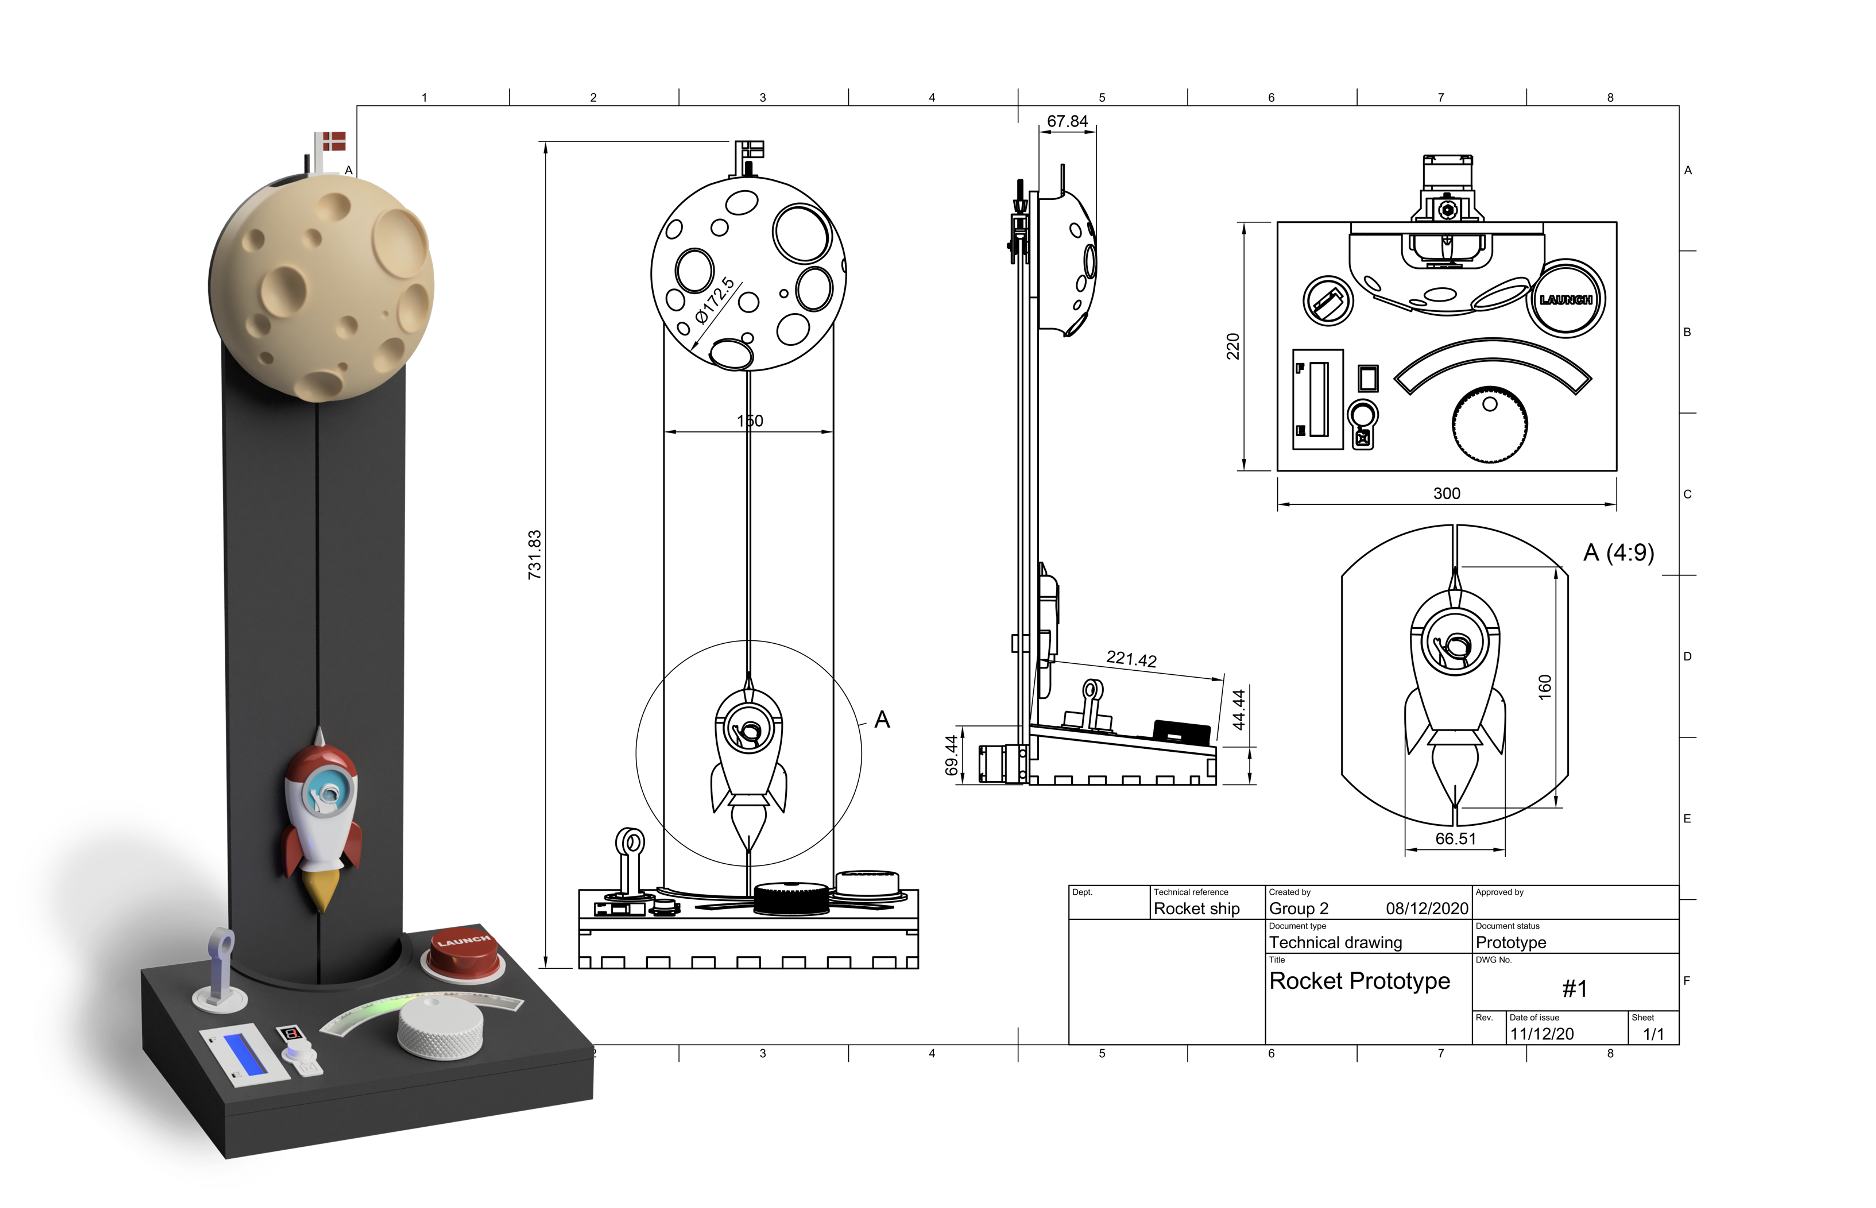
\includegraphics[width=\textwidth]{figure/sample.png}
  \caption{XXXXXX}
  \label{fig_XXXXXX}
\end{teaserfigure}

%% A "teaser" image could be added between the author and affiliation information and the body of the document.

\maketitle
\pagestyle{fancy}
\fancyhf{} % Clear the current header and footer
\fancyhead[L]{\fontsize{8}{9}\selectfont Example of Final Report: Lunar Shuttle - Stationary Moon Mission Toy}% Your project title
\fancyhead[R]{\fontsize{8}{9}\selectfont Group2} % The number of your group
\renewcommand{\headrulewidth}{0.1pt}
\fancyfoot[C]{\thepage} 
\renewcommand{\chaptermark}[1]{\markboth{#1}{}} %



\section{Introduction}
XXXXXX
%%In the introduction, provide a more comprehensive context for your prototype. Explain the background, real-world relevance, and motivation for undertaking this project. Clearly define the problem or challenge that your prototype addresses. Emphasize why this problem is worth solving and how your prototype contributes to solving it. Outline the specific objectives and goals your prototype aims to achieve.



\section{Related Works}
%In the related work section, delve deeper into the existing literature and projects that are relevant to your prototype. Analyze how prior research or projects have approached similar challenges and where they may have succeeded or fallen short. Highlight the uniqueness of your approach and discuss how your prototype either complements or innovates upon previous work.
XXXXXX \cite{djajadiningrat2004tangible}


\section{Prototype Design}
%In the design section, provide a detailed description of your prototype's architecture and components. Include detailed schematics, diagrams, or flowcharts to illustrate the design. Explain the rationale behind your design choices, including the selection of specific sensors, actuators, and microcontrollers. Describe the user interface and interaction model if applicable. Clarify how the design aligns with your project's objectives.
XXXXXX

\begin{figure}[t]
    \begin{subfigure}[t]{0.4\textwidth}
    \centering
        \includegraphics[width=\linewidth]{figure/XXXXXX}
        \caption{XXXXXX}
        \label{fig_XXXXXX}
    \end{subfigure}
    \begin{subfigure}[t]{0.4\textwidth}
        \centering
        \includegraphics[width=\linewidth]{figure/XXXXXX}
        \caption{XXXXXX}
        \label{fig_XXXXXX}
    \end{subfigure}
    \caption{XXXXXX}
    \label{fig_XXXXXX}
\end{figure}


\section{Main Components}
%This section could provide a step-by-step account of how you constructed the prototype. Describe the hardware assembly process, wiring, and connections in detail. Include code snippets and explain the logic and functionality of your software, emphasizing any unique algorithms or coding decisions. Discuss any challenges encountered during the implementation, technical problems faced, and how you overcame them. This section should provide readers with a clear guide on how to replicate your prototype.
XXXXXX

\begin{figure}[h]
  \centering
  \includegraphics[width=\linewidth]{figure/XXXXXX}
  \caption{XXXXXX}
  \label{fig_XXXXXX}
\end{figure}


\[
\frac{\text{XXXXXX}}{\text{XXXXXX}} = \text{XXXXXX}
\]


\section{Limitations and future work}
%In the limitations section, identify constraints or drawbacks of your prototype. These could include technical limitations, cost restrictions, or any design choices that may have affected the prototype's performance. Be honest about the areas where improvements or refinements could be made. The future work could outline potential enhancements and extensions for your prototype. Suggest areas where further development or research could lead to more robust solutions. Discuss how your prototype could be applied in different contexts or industries and what additional features or improvements.
XXXXXX


\section{Conclusion}
%In the conclusion, reiterate the main contributions and takeaways from your project. Summarize how your prototype addresses the identified problem or challenge. Discuss the broader implications of your work and its relevance in a larger context, such as how it can contribute to the advancement of the field of physical computing.
XXXXXX


\begin{table}
  \caption{Frequency of Special Characters}
  \label{tab:freq}
  \begin{tabular}{ccl}
    \toprule
    Non-English or Math&Frequency&Comments\\
    \midrule
    \O & 1 in 1,000& For Swedish names\\
    $\pi$ & 1 in 5& Common in math\\
    \$ & 4 in 5 & Used in business\\
    $\Psi^2_1$ & 1 in 40,000& Unexplained usage\\
  \bottomrule
\end{tabular}
\end{table}

\begin{table*}
  \caption{Some Typical Commands}
  \label{tab:commands}
  \begin{tabular}{ccl}
    \toprule
    Command &A Number & Comments\\
    \midrule
    \texttt{{\char'134}author} & 100& Author \\
    \texttt{{\char'134}table}& 300 & For tables\\
    \texttt{{\char'134}table*}& 400& For wider tables\\
    \bottomrule
  \end{tabular}
\end{table*}

% Always use midrule to separate table header rows from data rows, and
% use it only for this purpose. This enables assistive technologies to
% recognise table headers and support their users in navigating tables
% more easily.


%% The next two lines define the bibliography style to be used, and
%% the bibliography file.
\bibliographystyle{ACM-Reference-Format}
\bibliography{reference}


\appendix
%% If your work has an appendix, this is the place to put it. like code snippets, extensive data, or supplementary materials that are relevant to your report but would make the main text too lengthy, include them in the appendices.

\end{document}

